\begin{figure*}
  \center
  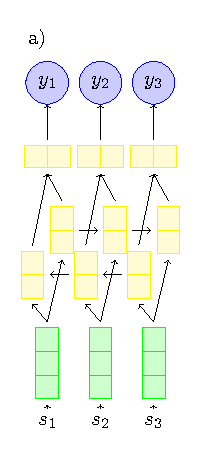
\includegraphics[scale=.7]{figures/rnnextractor.pdf}
  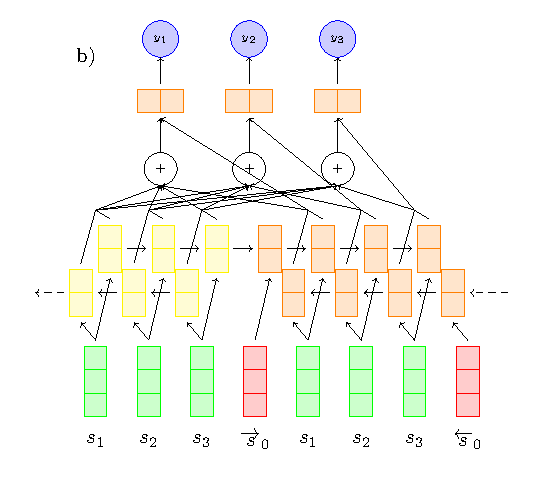
\includegraphics[scale=.7]{figures/s2s_extractor.pdf}
  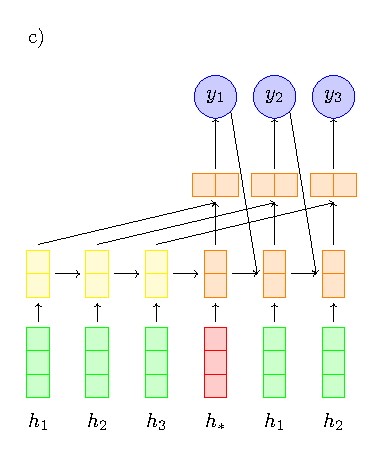
\includegraphics[scale=.7]{figures/clextractor.pdf}
  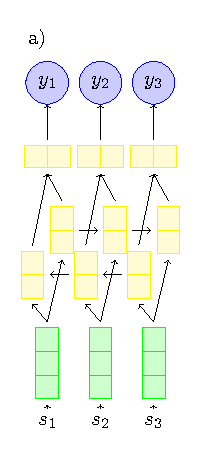
\includegraphics[scale=.7]{figures/rnnextractor.pdf}
  \caption{Sentence extractor architectures: a) RNN, b) Seq2Seq,
  c) Cheng \& Lapata, and d) SummaRunner. The $\bigoplus$ indicates 
  attention. Green repesents sentence encoder output, yellow and orange
  indicates
  extractor encoder and decoder hidden states respectively, and red indicates
  learned ``begin decoding'' embeddings. }
  \label{fig:extractors}
\end{figure*}

Given a sequence of sentence embeddings $\sentEmb = \sentEmb[1], \ldots, \sentEmb[\docSize]$ produced by a sentence encoder, 
a sentence extractor defines a conditional distribution $p(\slabel|\sentEmb)$
over the corresponding sentence extraction variables.

We first propose two simple extractor models based on bidirectional RNN 
and sequence-to-sequence with attention architectures, 
which we refer to as the RNN and 
Seq2Seq extractors respectively.

Next we define the extractor models of Cheng \& Lapata, and Nallapati et al.,
whose models we refer to as the Cheng \& Lapata and SummaRunner extractors
respectively.
See Figure~\ref{fig:extractors} for a diagram of the 
four sentence extractor architectures.



%$p(\slabel_1,\ldots,\slabel_{\sentSize}|\sentvec_1, \ldots, \sentvec_{\sentSize})$.
%We propose two simple recurrent neural network based sentence extractors
%that make a strong conditional independence assumption over the labels
%$\slabel_i$, namely
%$\explicitLikelihood= \naiveLikelihood$. This stands in contrast to our 
%baseline models which make a weaker assumption, \hal{this is really confusing cuz i don't think you've specified this yet, and it's still hard to understand what's new/yours and what's old/baseline.}
%$\compactLikelihood = \markovLikelihood$, at the expense of greater 
%computational complexity. 

\paragraph{RNN Extractor}
    Our first proposed model is a very simple bidirectional
RNN based tagging model. As in the RNN sentence encoder we use a GRU cell.
The  forward and backward outputs of each sentence are passed through a 
multi-layer perceptron with a logsitic sigmoid output (denoted by $\sigma$)
to predict the probability
of extracting each sentence. See details in Appendix~\ref{app:rnnextractor}

\begin{toappendix}
\section{Details on RNN Extractor.} \label{app:rnnextractor}
\begin{align}
    \rExtHidden_0 = \mathbf{0};&\quad   \rExtHidden_i = \rgru(\sentEmb[i], \rExtHidden_{i-1}) \\
    \lExtHidden_{\docSize + 1} = \mathbf{0};&\quad    \lExtHidden_i = \lgru(\sentEmb[i], \lExtHidden_{i+1}) \\
   \logits_i &= \relu\left(U \cdot [\rExtHidden_i; \lExtHidden_i] + u \right)\\
   p(\slabel_i=1|\sentvec) &= \sigma\left(V\cdot \logits_i + v  \right)
\end{align}
where $\rgru$ and $\lgru$ indicate the 
forward and backward GRUs respectively, and each have separate learned 
parameters; $U, V$ and $u, v$ are learned weight and bias parameters.
\end{toappendix}

\paragraph{\sts~Extractor} One shortcoming of the RNN extractor is that long range
information from one end of the document may not easily be able to effect 
extraction probabilities of sentences at the other end. 
Our second proposed model, the \sts~extractor mitigates this problem with an 
attention 
mechanism commonly
used for neural machine translation \cite{bahdanau2014neural} and 
abstractive summarization \cite{see2017get}. 
The sentence embeddings are first
encoded by a bidirectional $\gru$. A separate decoder $\gru$ transforms each 
sentence into a query vector which attends to the encoder output. The
attention weighted encoder output and the decoder $\gru$ output are concatenated
and fed into a multi-layer percepron to compute the extraction probability.
Detail in Appendix~\ref{app:s2sextractor}.
\begin{toappendix}
\section{Details on Seq2Seq Extractor.} \label{app:s2sextractor}
\begin{align}
    \rEncExtHidden_0 = \textbf{0}&;\quad \rEncExtHidden_i = \rgru_{enc}(\sentEmb[i], \rEncExtHidden_{i-1}) \\
    \lEncExtHidden_{\docSize + 1} = \textbf{0}&;\quad  \lEncExtHidden_i = \lgru_{enc}(\sentEmb[i], \lEncExtHidden_{i+1}) \\
    \rDecExtHidden_i &= \rgru_{dec}(\sentEmb[i], \rDecExtHidden_{i-1}) \\
    \lDecExtHidden_i &= \lgru_{dec}(\sentEmb[i], \lDecExtHidden_{i+1}) 
\end{align}
\begin{align}
 \decExtHidden_i = [\rDecExtHidden_i; \lDecExtHidden_i], &\;\;
 \encExtHidden_i = [\rEncExtHidden_i; \lEncExtHidden_i] 
\end{align}
\begin{align}
 \alpha_{i,j} = 
   \frac{\exp \left(\decExtHidden_i \cdot \encExtHidden_j \right)}{
   \sum_{j=1}^{\docSize}\exp\left(\decExtHidden_i \cdot \encExtHidden_j\right)}, 
& \;\; \attnExtHidden_i = \sum_{j=1}^{\docSize} \alpha_{i,j} \encExtHidden_j 
\end{align}
\begin{align}
   \logits_i = \relu\left(U \cdot [\attnExtHidden_i; \decExtHidden_i] + u \right)&\\
   p(\slabel_i=1|\sentvec) = \sigma\left(V\cdot \logits_i + v  \right).
\end{align}
The final outputs of each encoder direction are passed to the first decoder
steps; additionally, the first step of the decoder GRUs are learned 
``begin decoding'' vectors $\rDecExtHidden_0$ and $\lDecExtHidden_0$ 
(see Figure~\ref{fig:extractors}.b).
Each GRU has separate learned 
parameters; $U, V$ and $u, v$ are learned weight and bias parameters.
\end{toappendix}

\textbf{Cheng \& Lapata Extractor} 
We compare the previously proposed architectures to the sentence extractor
model of \cite{cheng2016neural}. 
%Unlike the previous models where
%sentence extraction predictions are conditionally independent given
%the sentence embeddings, this model uses previous extraction probabilities to
%influence later decisions. 

\begin{toappendix}
\section{Details on Cheng \& Lapata Extractor.} \label{app:clextractor}
The basic architecture is a unidirectional
sequence-to-sequence
model defined as follows:
\begin{align}
    \encExtHidden_0 = \textbf{0};&\quad   \encExtHidden_i = \gru_{enc}(\sentvec_i, \encExtHidden_{i-1}) \\
    \decExtHidden_1 &= \gru_{dec}(\sentEmb[*], \encExtHidden_{\docSize}) \\
    \decExtHidden_i &= \gru_{dec}(p_{i-1} \cdot \sentvec_{i-1}, \decExtHidden_{i-1}) \label{eq:cl1} \\
   \logits_i &= \relu\left(U \cdot [\encExtHidden_i; \decExtHidden_i] + u \right)\\
    p_i = p(\slabel_i&=1|\slabel_{<i}, \sentvec) = \sigma\left(V\cdot \logits_i + v  \right) 
\end{align}
where \sentEmb[*] is a learned ``begin decoding'' sentence embedding
(see Figure~\ref{fig:extractors}.c).
Each GRU has separate learned 
parameters; $U, V$ and $u, v$ are learned weight and bias parameters.
Note in Equation~\ref{eq:cl1} that 
the decoder side GRU input is the sentence embedding from the previous time
step weighted by its probabilitiy of extraction ($p_{i-1}$) from the 
previous step, inducing dependence of each output $y_i$ on all previous 
outputs $y_{<i}$.
\end{toappendix}

%\kathy{In many ways the Cheng and Lapata architecture looks simpler than yours. Can you indicate here why it is more complicated? Is it because of the number of learned parameters?}

Note that in the original paper, the Cheng \& Lapata extractor was paired 
with
a \textit{CNN} sentence encoder, but in this work we experiment with a variety
of sentence encoders.


\paragraph{SummaRunner Extractor}{
Our second baseline, which we refer to as the SummaRunner extractor is taken 
from 
\cite{nallapati2017summarunner}.



\begin{toappendix}
\section{Details on SummaRunner Extractor.} \label{app:srextractor}
Like the
\modelOne~extractor it starts with a bidrectional GRU over the sentence 
embeddings 
\begin{align}
    \rEncExtHidden_0 = \textbf{0}&;\quad \rEncExtHidden_i = \rgru(\sentvec_i, \rEncExtHidden_{i-1}) \\
    \lEncExtHidden_{\docSize + 1} = \textbf{0}&;\quad \lEncExtHidden_i = \lgru(\sentvec_i, \lEncExtHidden_{i+1}),
\end{align}
}

It then creates a representation
of the whole document $q$ by passing the averaged GRU output states through
a fully connected layer: 
\begin{align}
q = \tanh\left(b_q + W_q\frac{1}{\docSize}\sum_{i=1}^{\docSize} [\rEncExtHidden_i; \lEncExtHidden_i] \right)
\end{align}
A concatentation of the GRU outputs at each step
are passed through a separate fully connected layer to create a 
sentence representation $z_i$, where
\begin{align}
    \extHidden_i &= \relu\left(b_z + W_z [\rEncExtHidden_i; \lEncExtHidden_i]\right).
\end{align}
The extraction probability is then determined by contributions from five 
sources:
\begin{align}
    \textit{content} &\quad a^{(con)}_i=W^{(con)} z_i, \\
    \textit{salience}&\quad a^{(sal)}_i = z_i^TW^{(sal)} q, \\
    \textit{novelty}&\quad a^{(nov)}_i = -z_i^TW^{(nov)} \tanh(g_i), \label{eq:srnov} \\
    \textit{position}&\quad a^{(pos)}_i = W^{(pos)} l_i, \\
    \textit{quartile}&\quad a^{(qrt)}_i = W^{(qrt)} r_i,
\end{align}
where $l_i$ and $r_i$ are embeddings associated with the $i$-th sentence
position and the quarter of the document containing sentence $i$ respectively.
In Equation~\ref{eq:srnov}, $g_i$ is an iterative summary representation 
computed as the
sum of the previous $z_{<i}$ weighted by their extraction probabilities,
\begin{align}
g_i & = \sum_{j=1}^{i-1} p(y_j=1|y_{<j},h) \cdot z_j.
\end{align}
Note that the presence of this term induces dependence of each 
$\slabel_i$ to 
all $\slabel_{<i}$ similarly to the Cheng \& Lapata extractor.

The final extraction probability is the logistic sigmoid of the
sum of these terms plus a bias,
\begin{align}
    p(y_i=1|y_{<i}, h) &= \sigma\left(\begin{array}{l}
      a_i^{(con)} + a_i^{(sal)} + a_i^{(nov)} \\
  + a_i^{(pos)}  + a_i^{(qrt)} + b \end{array}\right).
\end{align}
The weight matrices $W_q$, $W_z$, $W^{(con)}$, $W^{(sal)}$, $W^{(nov)}$, $W^{(pos)}$,
$W^{(qrt)}$ and bias terms $b_q$, $b_z$, and $b$ are learned parameters;
The GRUs have separate learned parameters.
\end{toappendix}

Note that in the original paper, the SummaRunner extractor was paired 
with
an \textit{RNN} sentence encoder, but in this work we experiment with a variety
of sentence encoders.

%\begin{align}
%    \extHidden_i &= \relu\left(b_z + W_z [\rEncExtHidden_i; \lEncExtHidden_i]\right)
%  \end{align}
%  \begin{align*}
%      p(y_i=1|y_{<i}, h) = \sigma(& W_{con}\cdot z_i \\
%                     & + z_i^T W_{sal}\cdot q \\
%                     & -z_i^T W_{nov} \cdot \tanh(g_i) \\
%                     & + b_{rp_i}  \\
%                     & + b_{ap_i} \\
%                     & + b)     \\
%      g_j & = \sum_{i=1}^{j-1} p(y_j=1|y_{<j},h) \cdot z_j
%\end{align*}



%%% Local Variables:
%%% mode: latex
%%% TeX-master: "dlextsum.emnlp18"
%%% End:
